\documentclass[tikz,border=12pt]{standalone}
\usepackage[utf8]{inputenc}
\usepackage[T1]{fontenc}
\usepackage{amsmath,amssymb}
\usepackage{tikz}
\usepackage{pgfplots}
\pgfplotsset{compat=1.18}
\usepgfplotslibrary{groupplots}
\usetikzlibrary{arrows.meta,positioning,calc,backgrounds}

% V6 pastel-first palette
\definecolor{CoreNavy}{RGB}{72,92,120}
\definecolor{MutedBlue}{RGB}{104,132,164}
\definecolor{MutedRust}{RGB}{174,112,96}
\definecolor{MutedTeal}{RGB}{92,146,142}
\definecolor{PaleBlue}{RGB}{235,241,247}
\definecolor{PaleTeal}{RGB}{232,244,242}
\definecolor{PalePeach}{RGB}{248,238,231}
\definecolor{PaleRose}{RGB}{247,235,235}
\definecolor{SoftGray}{RGB}{244,245,246}
\definecolor{MidGray}{RGB}{153,160,168}
\definecolor{Ink}{RGB}{40,45,52}

\tikzset{
  module/.style={
    draw=CoreNavy,
    fill=SoftGray,
    line width=0.8pt,
    rounded corners=2mm,
    inner xsep=3.2mm,
    inner ysep=2.2mm,
    font=\sffamily\footnotesize,
    text=Ink,
    align=center
  }
}

\begin{document}
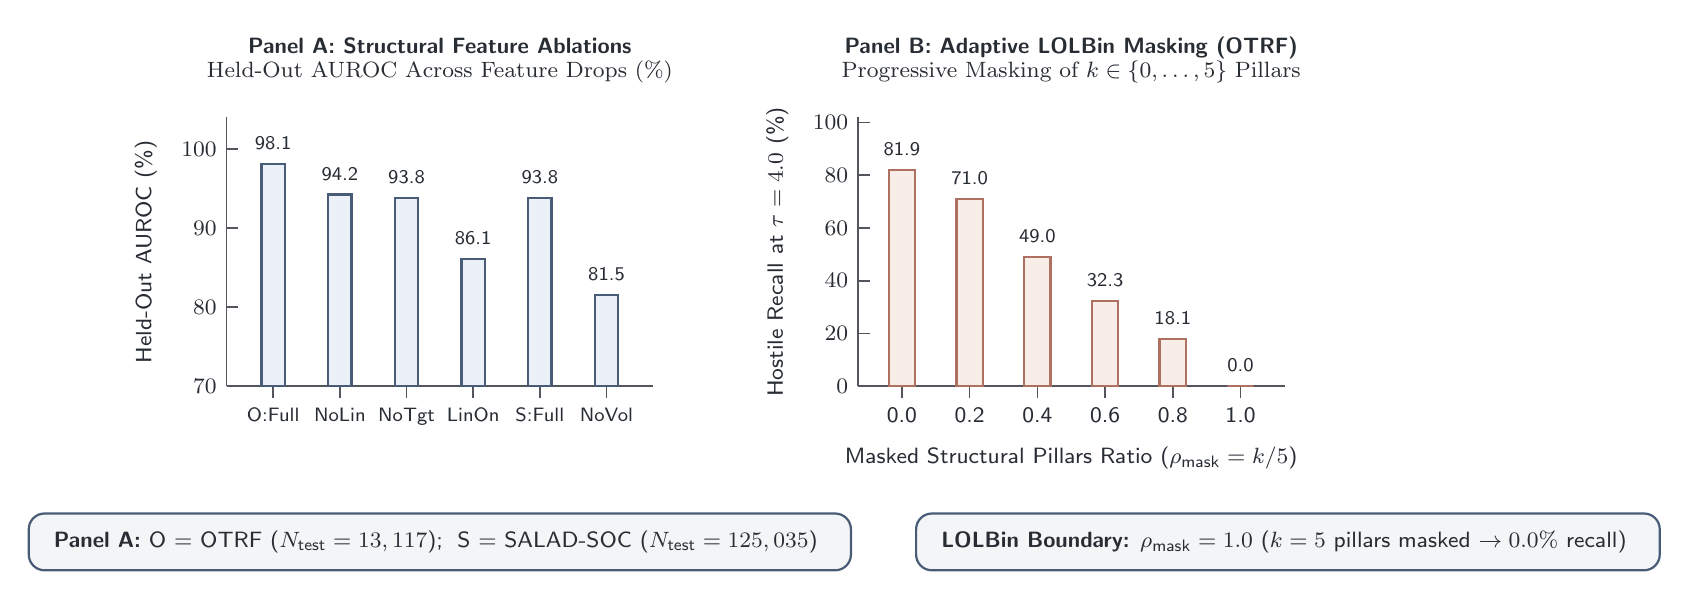
\begin{tikzpicture}[node distance=12mm and 14mm]

\begin{groupplot}[
  group style={
    group size=2 by 1,
    horizontal sep=26mm
  },
  width=70mm,
  height=50mm,
  grid=none,
  axis lines*=left,
  axis line style={draw=Ink!80, line width=0.7pt},
  tick style={draw=Ink!80, line width=0.6pt},
  tick label style={font=\sffamily\footnotesize, text=Ink},
  ylabel style={font=\sffamily\footnotesize, text=Ink, yshift=2pt},
  xlabel style={font=\sffamily\footnotesize, text=Ink, yshift=-2pt},
  title style={font=\sffamily\footnotesize\bfseries, text=Ink, align=center, yshift=3pt}
]

% Panel A: OTRF & SALAD-SOC Feature-Group Ablations (AUROC %)
\nextgroupplot[
  title={Panel A: Structural Feature Ablations\\[-1pt]\normalfont\footnotesize Held-Out AUROC Across Feature Drops (\%)},
  ylabel={Held-Out AUROC (\%)},
  ybar,
  ymin=70, ymax=104,
  ytick={70,80,90,100},
  symbolic x coords={OFull,ONoLin,ONoTgt,OLinOnly,SFull,SNoFlow},
  xtick={OFull,ONoLin,ONoTgt,OLinOnly,SFull,SNoFlow},
  xticklabels={O:Full,NoLin,NoTgt,LinOn,S:Full,NoVol},
  xticklabel style={align=center, font=\sffamily\scriptsize, text=Ink},
  enlarge x limits=0.14,
  point meta=explicit symbolic,
  nodes near coords,
  every node near coord/.append style={
    font=\sffamily\scriptsize,
    text=Ink,
    anchor=south,
    yshift=1.5pt
  }
]
\addplot[
  draw=CoreNavy,
  line width=0.85pt,
  fill=PaleBlue,
  bar width=8.5pt
] coordinates {
  (OFull,98.07) [98.1]
  (ONoLin,94.22) [94.2]
  (ONoTgt,93.78) [93.8]
  (OLinOnly,86.06) [86.1]
  (SFull,93.80) [93.8]
  (SNoFlow,81.51) [81.5]
};

% Panel B: Adaptive Attacker Structural Masking Curve on Held-Out OTRF
\nextgroupplot[
  title={Panel B: Adaptive LOLBin Masking (OTRF)\\[-1pt]\normalfont\footnotesize Progressive Masking of $k \in \{0,\dots,5\}$ Pillars},
  xlabel={Masked Structural Pillars Ratio ($\rho_{\text{mask}} = k/5$)},
  ylabel={Hostile Recall at $\tau=4.0$ (\%)},
  ybar,
  ymin=0, ymax=102,
  ytick={0,20,40,60,80,100},
  symbolic x coords={R00,R20,R40,R60,R80,R100},
  xtick={R00,R20,R40,R60,R80,R100},
  xticklabels={0.0,0.2,0.4,0.6,0.8,1.0},
  xticklabel style={align=center, font=\sffamily\footnotesize, text=Ink},
  enlarge x limits=0.13,
  point meta=explicit symbolic,
  nodes near coords,
  every node near coord/.append style={
    font=\sffamily\scriptsize,
    text=Ink,
    anchor=south,
    yshift=1.5pt
  }
]
\addplot[
  draw=MutedRust,
  line width=0.85pt,
  fill=PalePeach,
  bar width=9.5pt
] coordinates {
  (R00,81.94) [81.9]
  (R20,70.97) [71.0]
  (R40,49.03) [49.0]
  (R60,32.26) [32.3]
  (R80,18.06) [18.1]
  (R100,0.00) [0.0]
};

\end{groupplot}

% Relative summary nodes below panels
\node[module, below=16mm of group c1r1.south] (ab7_note) {
  \textbf{Panel A:} O = OTRF ($N_{\text{test}}=13,117$);\; S = SALAD-SOC ($N_{\text{test}}=125,035$)
};
\node[module, right=8mm of ab7_note] (lolbin_note) {
  \textbf{LOLBin Boundary:} $\rho_{\text{mask}}=1.0$ ($k=5$ pillars masked $\rightarrow 0.0\%$ recall)
};

\end{tikzpicture}
\end{document}
